\section{Problema 3: El se\~nor de los caballos}
\subsection{Descripci\'on de la problem\'atica}

En este problema, se presenta un tablero de ajedrez de tama\~no $nxn$, el cual cuenta con alguna cantidad de caballos ubicados en una posici\'on aleatoria del tablero. Lo que se quiere lograr es \emph{cubrir} todo el tablero. Un casillero se considera cubierto si hay un caballo en \'el o bien, si es una posici\'on en la cual alg\'un caballo existente puede moverse con un s\'olo movimiento. Para lograr este cometido, puede ser necesario agregar nuevas fichas \emph{caballo} al tablero. No existe un l\'imite en la cantidad de caballos para agregar, pero lo que se busca es dar una soluci\'on agregando la menor cantidad de caballos posibles.\\

 \begin{figure}[h!]
   \begin{center}
 	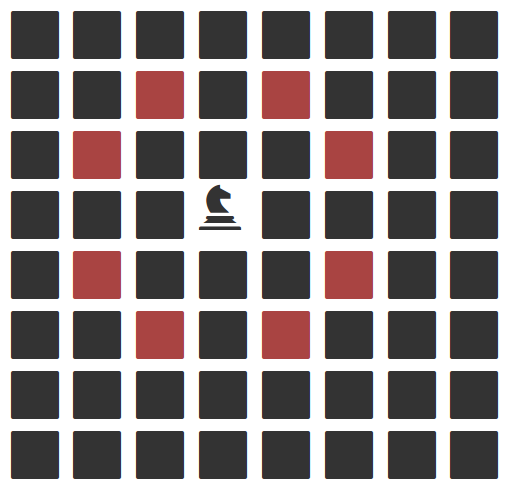
\includegraphics[scale=0.4]{imagenes/ej3/unCaballo.png}
 	\caption{Casillas que \emph{cubre} un caballo}
   \end{center}
 \end{figure}

 \begin{figure}[h!]
   \begin{center}
 	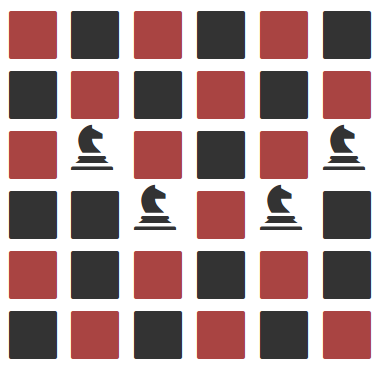
\includegraphics[width=.4\linewidth]{imagenes/ej3/6x6init.png}
 	\caption{As\'i se ve un tablero en un posible estado inicial}
   \end{center}
 \end{figure}

 \begin{figure}[h!]
   \begin{center}
 	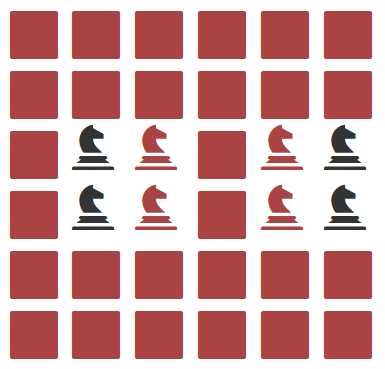
\includegraphics[width=.4\linewidth]{imagenes/ej3/6x6optima.png}
 	\caption{Y esta ser\'ia una de las soluciones \'optimas donde se el agregan 4 caballos}
   \end{center}
 \end{figure}

\newpage

\subsection{Resoluci\'on propuesta y justificaci\'on}
Para la resoluci\'on de este ejercicio, se ped\'ia un algoritmo de backtracking. O sea que el algortimo debe, a partir de una subsoluci\'on del problema, fijarse si es soluci\'on y hacer algo  al respecto con ella, o bien si es una subsoluci\'on v\'alida, para cada elemento que se pueda agregar a la subsoluci\'on, agregarselo y repetir el proceso, o en el \'ultimo caso, si se llega a una soluci\'on no v\'alida, volver hacia atr\'as y tomar una decisi\'on adecuada. Esto implica que el algortimo debe revisar un extenso \'arbol de posibilidades, donde una decisi\'on es agregar o no un caballo en la posici\'on $i, j$ del tablero para todo $i, j$ dentro del rango del mismo. Posterior a esto se ped\'ia pensar e implementar una serie de podas y estrategias para no recorrer todo el \'arbol, sino mirarlo inteligentemente y as\'i reducir los tiempos de ejecuci\'on.\\

El algortimo es muy sencillo, pregunta cu\'antos caballos hace falta agregar para cubrir el tablero si en la posici\'on $i, j$ agrega un caballo (recursivamente llena todo el tablero) y lo compara con la respuesta de no agregarlo, qued\'andose siempre con la soluci\'on que menos caballos extra le lleva.\\

El algoritmo resuelve el ejercicio planteado porque recorre todo el \'arbol de soluciones y se queda con alguna de las m\'as \'optimas.\\

\textcolor{blue}{Como que no pude cerrar la idea... AYUDA}

\newpage

\subsection{An\'alisis de la complejidad}
Para analizar la complejidad de este algoritmo, hay que tener en cuenta dos situaciones.\\

Sea n = dimensi\'on del tablero\\

Si el tablero viene cubierto por los caballos preubicados, entonces el algoritmo chequea esto y devuelve que est\'a completo en tiempo $O(n^{2})$, es decir, recorrer la matriz donde est\'a almacenado el tablero, posici\'on por posici\'on.\\

Si no empieza a trabajar con el backtracking. El primer approach para la resoluci\'on del ejercicio fue aplicar "fuerza bruta", d\'andonos una complejidad de $O(2^{n^{2} - k})$ siendo k la cantidad de caballos preubicados. Esto es para cada posici\'on sin caballos, ver que pasa si tomo alguna de las dos posibles decisiones, o lo que es lo mismo, recorrer por completo el \'arbol de soluciones y devolver la de m\'as \'optima.\\

Para disminuir los tiempos de ejecuci\'on (en otra secci\'on se hablar\'a sobre esto) se pidi\'o realizar podas al \'arbol y estrategias de recorrido (determinar si vale la pena o no seguir revisando alguna rama).\\

Ninguna poda/estrategia disminuye la complejidad te\'orica exponencial del primer approach, dado que el algoritmo realiza las mismas preguntas para cada posici\'on del tablero, ¿qu\'e pasa si lo dejo sin caballo? ¿qu\'e pasa si le pongo un caballo?. No obstante, los tiempos de ejecuci\'on se ven radicalmente afectados, esto sucede porque se poda el \'arbol de soluciones posibles que se analizan, es decir, en el primer approach, se revisan todas las ramas, sin excepci\'on, y aplicando podas descartamos muchas de estas que ya sabemos que no nos llevar\'an a un resultado que nos interese.\\


La primera poda fue la m\'as intuitiva, si tenemos una soluci\'on con k caballos extra agregados,  y analizando otra rama llegamos a tener que necesitar agregar un caballo a una subsoluci\'on de k-1 caballos (o sea que tendr\'ia por lo menos k caballos), entonces no nos interesa seguir revis\'andola, pues tenemos una soluci\'on que es igual o m\'as \'optima con k caballos.\\

La segunda estrategia fue plantear si en alg\'un momento sab\'iamos que no deb\'iamos agregar un caballo en un determinado casillero. Entonces, salteamos las k posiciones de los caballos preubicados y adem\'as salteamos aquellas posiciones que, estando atacadas, si le pusieramos un caballo, estar\'ian atancando a casilleros que ya est\'an siendo cubiertos por otros caballos.\\

\newpage

\subsection{C\'odigo fuente}
\newpage
\subsection{Experimentaci\'on}

\subsubsection*{Constrastaci\'on Emp\'irica de la complejidad}
-Hacer lo que hicieron en clase\\
\newpage
